% answers.tex —— 2012 年·天津卷·文科 · 参考答案与详细解析片段
% 由 tools/generate_projects.py 依来源总账自 2012/2012_数学真题_天津文_试题.md + 2012/2012_数学真题_天津文_解析正文.md + 2012/2012_数学真题_天津文_答案要点.md 生成，勿手改（改源 MD 后重跑）

\begin{answer}
\gksolhead{1}{}

\textbf{题目}：

$\mathrm i$ 是虚数单位，复数 $\dfrac{5+3\mathrm i}{4-\mathrm i}=$\mbox{（　　）}

（A）$1-\mathrm i$；（B）$-1+\mathrm i$；（C）$1+\mathrm i$；（D）$-1-\mathrm i$。

\Needspace{4\baselineskip}
\textbf{解析}
\nopagebreak[4]
\[\frac{5+3\mathrm i}{4-\mathrm i}=\frac{(5+3\mathrm i)(4+\mathrm i)}{17}=\frac{17+17\mathrm i}{17}=1+\mathrm i.\]
选 C。

\gkanswer{答案：C。}

\end{answer}
\begin{answer}
\gksolhead{2}{}

\textbf{题目}：

设变量 $x$，$y$ 满足约束条件 $\begin{cases}2x+y-2\geqslant0,\\ x-2y+4\geqslant0,\\ x-1\leqslant0,\end{cases}$ 则目标函数 $z=3x-2y$ 的最小值为\mbox{（　　）}

（A）$-5$；（B）$-4$；（C）$-2$；（D）$3$。

\Needspace{4\baselineskip}
\textbf{解析}
可行域顶点为 $(0,2)$，$\left(1,\dfrac52\right)$，$(1,0)$。$z=3x-2y$ 在三点处分别为 $-4$，$-2$，$3$，故最小值为 $-4$。选 B。

\gkanswer{答案：B。}

\end{answer}
\begin{answer}
\gksolhead{3}{}

\textbf{题目}：

阅读如图程序框图，运行相应的程序，则输出 $S$ 的值为\mbox{（　　）}
\nopagebreak[4]
\begin{center}% 2012 年天津卷文科第 3 题：程序框图（n=1,S=0；S=S+3^n-3^{n-1}；n=n+1；n>=4 输出 S）
% 来源 PDF：普通高考/2012/2012天津文.pdf，第 1 页（印面 777）第 1 栏。
\begin{tikzpicture}[scale=0.9, semithick, >=Stealth,
  block/.style={draw, minimum width=3.4cm, minimum height=0.7cm, align=center},
  dec/.style={draw, diamond, aspect=3.0, inner sep=1pt, align=center},
  arr/.style={->}]
  \node (start) [draw, rounded corners=6pt, minimum width=1.5cm, minimum height=0.55cm] {开始};
  \node (init)  [block, below=0.5cm of start] {$n=1,\ S=0$};
  \node (step)  [block, below=0.6cm of init] {$S=S+3^n-3^{n-1}$};
  \node (inc)   [block, below=0.55cm of step] {$n=n+1$};
  \node (dec)   [dec, below=0.7cm of inc] {$n\geqslant4$?};
  \node (out)   [draw, trapezium, trapezium left angle=70, trapezium right angle=110,
                 minimum width=2.6cm, minimum height=0.65cm, below=0.8cm of dec] {输出 $S$};
  \node (end)   [draw, rounded corners=6pt, minimum width=1.5cm, minimum height=0.55cm,
                 below=0.5cm of out] {结束};
  \draw[arr] (start) -- (init);
  \draw[arr] (init) -- (step);
  \draw[arr] (step) -- (inc);
  \draw[arr] (inc) -- (dec);
  \draw[arr] (dec) -- node[right] {是} (out);
  \draw[arr] (out) -- (end);
  \draw[arr] (dec.east) -- node[above] {否} ++(1.7,0) |- (init.east);
\end{tikzpicture}
\end{center}
\nopagebreak[4]
（A）$8$；（B）$18$；（C）$26$；（D）$80$。

\Needspace{4\baselineskip}
\textbf{解析}
$n=1$：$S=0+3^1-3^0=2$，$n=2$；$2<4$：$S=2+9-3=8$，$n=3$；$3<4$：$S=8+27-9=26$，$n=4$；$4\geqslant4$，输出 $26$。选 C。

\gkanswer{答案：C。}

\end{answer}
\begin{answer}
\gksolhead{4}{}

\textbf{题目}：

已知 $a=2^{1.2}$，$b=\left(\dfrac12\right)^{-0.8}$，$c=2\log_25$，则 $a$，$b$，$c$ 的大小关系为\mbox{（　　）}

（A）$c<b<a$；（B）$c<a<b$；（C）$b<a<c$；（D）$b<c<a$。

\Needspace{4\baselineskip}
\textbf{解析}
$b=2^{0.8}$，$a=2^{1.2}$，$c=2\log_25=\log_2 25>4$，故 $c>a>b$。选 A。

\gkanswer{答案：A。}

\end{answer}
\begin{answer}
\gksolhead{5}{}

\textbf{题目}：

设 $x\in\mathbf R$，则「$x>\dfrac12$」是「$2x^2+x-1>0$」的\mbox{（　　）}

（A）充分而不必要条件；（B）必要而不充分条件；（C）充分必要条件；（D）既不充分也不必要条件。

\Needspace{4\baselineskip}
\textbf{解析}
$2x^2+x-1>0\iff(2x-1)(x+1)>0\iff x>\dfrac12$ 或 $x<-1$。故 $x>\dfrac12$ 充分而不必要。选 A。

\gkanswer{答案：A。}

\end{answer}
\begin{answer}
\gksolhead{6}{}

\textbf{题目}：

下列函数中，既是偶函数，又在区间 $(1,2)$ 内是增函数的是\mbox{（　　）}

（A）$y=\cos2x$，$x\in\mathbf R$；（B）$y=\log_2|x|$，$x\in\mathbf R$ 且 $x\neq0$；

（C）$y=\dfrac{\mathrm e^x-\mathrm e^{-x}}2$，$x\in\mathbf R$；（D）$y=x^3+1$，$x\in\mathbf R$。

\Needspace{4\baselineskip}
\textbf{解析}
（A）$\cos2x$ 在 $(1,2)$ 内不单调；（C）为奇函数；（D）非偶函数；（B）$y=\log_2|x|$ 为偶函数且在 $(0,+\infty)$ 递增。选 B。

\gkanswer{答案：B。}

\end{answer}
\begin{answer}
\gksolhead{7}{}

\textbf{题目}：

将函数 $f(x)=\sin\omega x$（其中 $\omega>0$）的图象向右平移 $\dfrac\pi4$ 个单位长度，所得图象经过点 $\left(\dfrac{3\pi}4,0\right)$，则 $\omega$ 的最小值是\mbox{（　　）}

（A）$\dfrac13$；（B）$1$；（C）$\dfrac53$；（D）$2$。

\Needspace{4\baselineskip}
\textbf{解析}
\Needspace{5\baselineskip}
平移后 $y=\sin\left(\omega x-\dfrac{\omega\pi}4\right)$，代入 $\left(\dfrac{3\pi}4,0\right)$：
\nopagebreak[4]
\[\sin\left(\frac{\omega\pi}2\right)=0\Longrightarrow\frac{\omega\pi}2=k\pi\Longrightarrow\omega=2k\ (k\in\mathbf N^*),\]
故 $\omega$ 的最小值为 $2$。选 D。

\gkanswer{答案：D。}

\end{answer}
\begin{answer}
\gksolhead{8}{}

\textbf{题目}：

在 $\triangle ABC$ 中，$\angle A=90^\circ$，$AB=1$，$AC=2$。设点 $P$，$Q$ 满足 $\overrightarrow{AP}=\lambda\overrightarrow{AB}$，$\overrightarrow{AQ}=(1-\lambda)\overrightarrow{AC}$，$\lambda\in\mathbf R$。若 $\overrightarrow{BQ}\cdot\overrightarrow{CP}=-2$，则 $\lambda=$\mbox{（　　）}

（A）$\dfrac13$；（B）$\dfrac23$；（C）$\dfrac43$；（D）$2$。

\Needspace{4\baselineskip}
\textbf{解析}
\Needspace{5\baselineskip}
以 $A$ 为原点，$AB$，$AC$ 为 $x$，$y$ 轴：$B(1,0)$，$C(0,2)$，$P(\lambda,0)$，$Q(0,2(1-\lambda))$。
\nopagebreak[4]
\[\overrightarrow{BQ}=(-1,2(1-\lambda)),\qquad\overrightarrow{CP}=(\lambda,-2),\]
\nopagebreak[4]
\[\overrightarrow{BQ}\cdot\overrightarrow{CP}=-\lambda-4(1-\lambda)=3\lambda-4=-2\Longrightarrow\lambda=\frac23.\]
选 B。

\gkanswer{答案：B。}

\end{answer}
\begin{answer}
\gksolhead{9}{}

\textbf{题目}：

集合 $A=\{x\in\mathbf R\mid |x-2|\leqslant5\}$ 中的最小整数为\gkblank{}。

\Needspace{4\baselineskip}
\textbf{解析}
$|x-2|\leqslant5$ 即 $-3\leqslant x\leqslant7$，最小整数为 $-3$。

\gkanswer{答案：$-3$。}

\end{answer}
\begin{answer}
\gksolhead{10}{}

\textbf{题目}：

一个几何体的三视图如图所示（单位：$\mathrm m$），则该几何体的体积为\gkblank{}$\mathrm{m}^3$。
\nopagebreak[4]
\begin{center}% 2012 年天津卷文科第 10 题：三视图（单位：m）
% 来源 PDF：普通高考/2012/2012天津文.pdf，第 1 页（印面 777）第 2 栏。
% 重绘依据：正视图为 3×2 矩形，上方直角梯形（下底 2、上底 1、高 1）；
%   侧视图为 4×3 矩形，y=2 处一条横线；俯视图 3×4，x=1、x=2 两条竖线。
\begin{tikzpicture}[scale=0.72, semithick, every node/.style={font=\small}]
  % ---------- 正视图 ----------
  \begin{scope}[shift={(0,0)}]
    \draw (0,0) rectangle (3,2);
    \draw (1,2) -- (2,3) -- (3,3) -- (3,2);
    \draw[<->] (0,-0.3) -- (3,-0.3) node[midway,below] {$3$};
    \draw[<->] (3.45,0) -- (3.45,2) node[midway,right] {$2$};
    \draw[<->] (3.45,2) -- (3.45,3) node[midway,right] {$1$};
    \draw[densely dashed] (0,2) -- (1,2);
    \node at (1.5,-1.0) {正视图};
  \end{scope}
  % ---------- 侧视图 ----------
  \begin{scope}[shift={(5.6,0)}]
    \draw (0,0) rectangle (4,3);
    \draw (0,2) -- (4,2);
    \draw[<->] (0,-0.3) -- (4,-0.3) node[midway,below] {$4$};
    \draw[<->] (4.45,0) -- (4.45,2) node[midway,right] {$2$};
    \draw[<->] (4.45,2) -- (4.45,3) node[midway,right] {$1$};
    \node at (2,-1.0) {侧视图};
  \end{scope}
  % ---------- 俯视图 ----------
  \begin{scope}[shift={(0,-5.2)}]
    \draw (0,0) rectangle (3,4);
    \draw (1,0) -- (1,4);
    \draw (2,0) -- (2,4);
    \draw[<->] (0,-0.3) -- (1,-0.3) node[midway,below] {$1$};
    \draw[<->] (1,-0.3) -- (2,-0.3) node[midway,below] {$1$};
    \draw[<->] (2,-0.3) -- (3,-0.3) node[midway,below] {$1$};
    \draw[<->] (3.45,0) -- (3.45,4) node[midway,right] {$4$};
    \node at (1.5,-1.0) {俯视图};
  \end{scope}
\end{tikzpicture}
\end{center}
\nopagebreak[4]
\Needspace{4\baselineskip}
\textbf{解析}
\Needspace{5\baselineskip}
由三视图：下部是 $3\times4\times2$ 的长方体；上部是横截面为直角梯形（下底 $2$、上底 $1$、高 $1$）、纵深 $4$ 的柱体。
\nopagebreak[4]
\[V=3\times4\times2+\frac{(2+1)\times1}2\times4=24+6=30.\]

\gkanswer{答案：$30$。}

\end{answer}
\begin{answer}
\gksolhead{11}{}

\textbf{题目}：

已知双曲线 $C_1:\dfrac{x^2}{a^2}-\dfrac{y^2}{b^2}=1$（$a>0$，$b>0$）与双曲线 $C_2:\dfrac{x^2}4-\dfrac{y^2}{16}=1$ 有相同的渐近线，且 $C_1$ 的右焦点为 $F(\sqrt5,0)$，则 $a=$\gkblank{}，$b=$\gkblank{}。

\Needspace{4\baselineskip}
\textbf{解析}
$C_2$ 的渐近线为 $y=\pm2x$，故 $\dfrac ba=2$。右焦点 $(\sqrt5,0)$ 给出 $a^2+b^2=5$，结合 $b=2a$ 得 $5a^2=5$，$a=1$，$b=2$。

\gkanswer{答案：$a=1$，$b=2$。}

\end{answer}
\begin{answer}
\gksolhead{12}{}

\textbf{题目}：

设 $m$，$n\in\mathbf R$，若直线 $l:mx+ny-1=0$ 与 $x$ 轴相交于点 $A$，与 $y$ 轴相交于点 $B$，且 $l$ 与圆 $x^2+y^2=4$ 相交所得弦的长为 $2$，$O$ 为坐标原点，则 $\triangle AOB$ 面积的最小值为\gkblank{}。

\Needspace{4\baselineskip}
\textbf{解析}
\Needspace{5\baselineskip}
直线与圆相交所得弦长为 $2$，圆半径为 $2$，故圆心到直线距离为 $\sqrt{4-1}=\sqrt3$，即
\nopagebreak[4]
\[\frac1{\sqrt{m^2+n^2}}=\sqrt3\Longrightarrow m^2+n^2=\frac13.\]
\Needspace{5\baselineskip}
$A\left(\dfrac1m,0\right)$，$B\left(0,\dfrac1n\right)$，故
\nopagebreak[4]
\[S_{\triangle AOB}=\frac1{2|mn|}\geqslant\frac1{m^2+n^2}=\frac1{1/3}=3,\]
当 $|m|=|n|$ 时取等号。

\gkanswer{答案：$3$。}

\end{answer}
\begin{answer}
\gksolhead{13}{}

\textbf{题目}：

已知 $AB$ 和 $AC$ 是圆的两条弦，过点 $B$ 作圆的切线与 $AC$ 的延长线相交于点 $D$。过点 $C$ 作 $BD$ 的平行线与圆相交于点 $E$，与 $AB$ 相交于点 $F$，$AF=3$，$FB=1$，$EF=\dfrac32$，则线段 $CD$ 的长为\gkblank{}。
\nopagebreak[4]
\begin{center}% 2012 年天津卷文科第 13 题：AB、AC 为圆的两条弦，过 B 的切线交 AC 延长线于 D，
% 过 C 作 BD 的平行线交圆于 E、交 AB 于 F。
% 来源 PDF：普通高考/2012/2012天津文.pdf，第 1 页（印面 777）第 2 栏。
% 重绘依据：按 AF=3、FB=1、EF=3/2 反算圆半径 R=sqrt(64/15)≈2.066，
%   A(-2,0.516)、B(2,0.516)、C(1.5,-1.420)、E(0.625,1.969)、D(2.667,-2.066)。
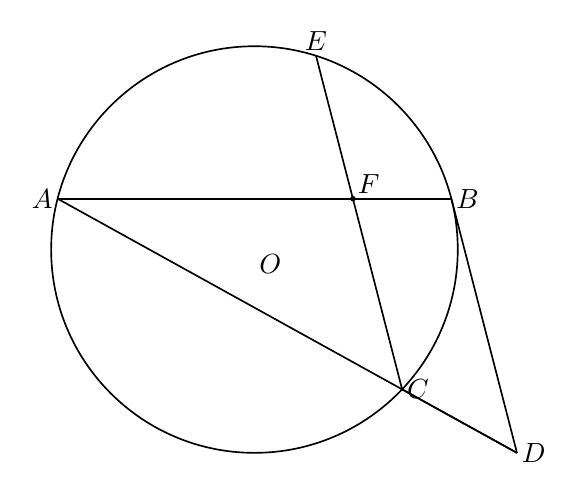
\begin{tikzpicture}[scale=1.25, semithick, every node/.style={inner sep=1.5pt}]
  \coordinate (O) at (0,0);
  \draw (O) circle (2.0656);
  \coordinate (A) at (-2,0.5164);
  \coordinate (B) at (2,0.5164);
  \coordinate (C) at (1.5,-1.4201);
  \coordinate (E) at (0.625,1.9688);
  \coordinate (F) at (1,0.5164);
  \coordinate (D) at (2.6667,-2.0656);
  \draw (A) -- (B);
  \draw (A) -- (D);
  \draw (C) -- (D);
  \draw (B) -- (D);
  \draw (C) -- (E);
  \fill (F) circle (0.8pt);
  \node[left] at (A) {$A$};
  \node[right] at (B) {$B$};
  \node[right] at (C) {$C$};
  \node[right] at (D) {$D$};
  \node[above] at (E) {$E$};
  \node[above right] at (F) {$F$};
  \node[below right] at (O) {$O$};
\end{tikzpicture}
\end{center}
\nopagebreak[4]
\Needspace{4\baselineskip}
\textbf{解析}
\Needspace{5\baselineskip}
在 $\triangle ABD$ 中，$C$ 在 $AD$ 上，$F$ 在 $AB$ 上，且 $CF\parallel BD$，故
\nopagebreak[4]
\[\frac{AF}{AB}=\frac{AC}{AD}=\frac{CF}{BD}.\]
由 $AF=3$，$AB=4$ 得 $\dfrac{AC}{AD}=\dfrac34$，即 $AD=\dfrac43AC$，$CD=\dfrac13AC$。
\Needspace{5\baselineskip}
由相交弦定理 $FA\cdot FB=FE\cdot FC$，即 $3\times1=\dfrac32\cdot FC$，得 $FC=2$，从而
\nopagebreak[4]
\[BD=\frac43CF=\frac83.\]
\Needspace{5\baselineskip}
由切割线定理 $BD^2=DC\cdot DA$：
\nopagebreak[4]
\[\left(\frac83\right)^2=\frac{AC}3\cdot\frac{4AC}3=\frac{4AC^2}9\Longrightarrow AC=4,\]
故 $CD=\dfrac{AC}3=\dfrac43$。

\gkanswer{答案：$\dfrac43$。}

\end{answer}
\begin{answer}
\gksolhead{14}{}

\textbf{题目}：

已知函数 $y=\dfrac{|x^2-1|}{x-1}$ 的图象与函数 $y=kx$ 的图象恰有两个交点，则实数 $k$ 的取值范围是\gkblank{}。

\Needspace{4\baselineskip}
\textbf{解析}
当 $x>1$ 时 $y=x+1$；当 $x<1$ 时 $y=-(x+1)$（$x=-1$ 时 $y=0$）。
与 $y=kx$ 联立：$x>1$ 时 $x=\dfrac1{k-1}>1\iff0<k<1$；$x<1$ 时 $x=-\dfrac1{k+1}<1$。
恰有两个交点必须两类各一个：$0<k<1$ 时 $x<1$ 的解为 $-\dfrac1{k+1}\in\left(-\infty,-\dfrac12\right)<1$ ；$k\leqslant0$ 时第一类无解。故 $k\in(0,1)$。

\gkanswer{答案：$(0,1)$。}

\end{answer}
\begin{answer}
\gksolhead{15}{}

\textbf{题目}：

某地区有小学 $21$ 所，中学 $14$ 所，大学 $7$ 所，现采用分层抽样的方法从这些学校中抽取 $6$ 所学校对学生进行视力调查。

（1） 求应从小学、中学、大学中分别抽取的学校数目；

（2） 若从抽取的 $6$ 所学校中随机抽取 $2$ 所学校做进一步数据分析，
① 列出所有可能的抽取结果；
② 求抽取的 $2$ 所学校均为小学的概率。

\Needspace{4\baselineskip}
\textbf{解析}
\textbf{（1）} 总校数 $21+14+7=42$，抽样比 $\dfrac6{42}=\dfrac17$，故小学 $21\times\dfrac17=3$ 所，中学 $14\times\dfrac17=2$ 所，大学 $7\times\dfrac17=1$ 所。

\textbf{（2）} ① 记 $3$ 所小学为 $A_1,A_2,A_3$，$2$ 所中学为 $B_1,B_2$，$1$ 所大学为 $C$。任取 $2$ 所的所有结果为
$A_1A_2$，$A_1A_3$，$A_1B_1$，$A_1B_2$，$A_1C$，$A_2A_3$，$A_2B_1$，$A_2B_2$，$A_2C$，$A_3B_1$，$A_3B_2$，$A_3C$，$B_1B_2$，$B_1C$，$B_2C$，共 $15$ 种。
② 两所均为小学的结果有 $A_1A_2$，$A_1A_3$，$A_2A_3$ 共 $3$ 种，概率为 $\dfrac3{15}=\dfrac15$。

\gkanswer{答案（1）：小学 $3$ 所，中学 $2$ 所，大学 $1$ 所。}

\gkanswer{答案（2）：① 见解析（共 $15$ 种）；② $\dfrac15$。}

\end{answer}
\begin{answer}
\gksolhead{16}{}

\textbf{题目}：

在 $\triangle ABC$ 中，内角 $A$，$B$，$C$ 所对的边分别是 $a$，$b$，$c$。已知 $a=2$，$c=\sqrt2$，$\cos A=-\dfrac{\sqrt2}4$。

（1） 求 $\sin C$ 和 $b$ 的值；

（2） 求 $\cos\left(2A+\dfrac\pi3\right)$ 的值。

\Needspace{4\baselineskip}
\textbf{解析}
\Needspace{5\baselineskip}
\textbf{（1）} $\sin A=\sqrt{1-\dfrac18}=\dfrac{\sqrt{14}}4$。由正弦定理
\nopagebreak[4]
\[\sin C=\frac{c\sin A}a=\frac{\sqrt2\cdot\frac{\sqrt{14}}4}2=\frac{\sqrt7}4.\]
\Needspace{5\baselineskip}
因 $\cos A<0$，$A$ 为钝角，故 $C$ 为锐角，$\cos C=\sqrt{1-\dfrac7{16}}=\dfrac34$。由射影定理
\nopagebreak[4]
\[b=a\cos C+c\cos A=2\cdot\frac34+\sqrt2\cdot\left(-\frac{\sqrt2}4\right)=\frac32-\frac12=1.\]

\Needspace{5\baselineskip}
\textbf{（2）}
\nopagebreak[4]
\[\cos2A=2\cos^2A-1=2\cdot\frac18-1=-\frac34,\qquad \sin2A=2\sin A\cos A=2\cdot\frac{\sqrt{14}}4\cdot\left(-\frac{\sqrt2}4\right)=-\frac{\sqrt7}4.\]
\nopagebreak[4]
\[\cos\left(2A+\frac\pi3\right)=\frac12\cos2A-\frac{\sqrt3}2\sin2A=-\frac38+\frac{\sqrt{21}}8=\frac{\sqrt{21}-3}8.\]

\gkanswer{答案（1）：$\sin C=\dfrac{\sqrt7}4$，$b=1$。}

\gkanswer{答案（2）：$\dfrac{\sqrt{21}-3}8$。}

\end{answer}
\begin{answer}
\gksolhead{17}{}

\textbf{题目}：

如图，在四棱锥 $P-ABCD$ 中，底面 $ABCD$ 是矩形，$AD\perp PD$，$BC=1$，$PC=2\sqrt3$，$PD=CD=2$。

（1） 求异面直线 $PA$ 与 $BC$ 所成角的正切值；

（2） 证明：平面 $PDC\perp$ 平面 $ABCD$；

（3） 求直线 $PB$ 与平面 $ABCD$ 所成角的正弦值。
\nopagebreak[4]
\begin{center}% 2012 年天津卷文科第 17 题：四棱锥 P-ABCD，底面 ABCD 为矩形，AD⊥PD。
% 来源 PDF：普通高考/2012/2012天津文.pdf，第 2 页（印面 778）第 1 栏。
% 重绘依据：原图为斜二测式透视：A、B 在前，C、D 在后，P 在上方偏左；
%   实线 PA、PB、PC、PD、AB、BC，虚线 AD、CD、AC。
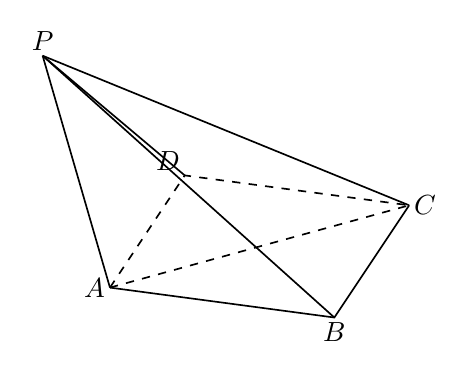
\begin{tikzpicture}[scale=0.95, semithick, every node/.style={inner sep=1.5pt}]
  \coordinate (A) at (0.4,0.5);
  \coordinate (B) at (3.4,0.1);
  \coordinate (C) at (4.4,1.6);
  \coordinate (D) at (1.4,2.0);
  \coordinate (P) at (-0.5,3.6);
  \draw (P) -- (A);
  \draw (P) -- (B);
  \draw (P) -- (C);
  \draw (P) -- (D);
  \draw (A) -- (B) -- (C);
  \draw[dashed] (A) -- (D) -- (C);
  \draw[dashed] (A) -- (C);
  \node[left] at (A) {$A$};
  \node[below] at (B) {$B$};
  \node[right] at (C) {$C$};
  \node[above left] at (D) {$D$};
  \node[above] at (P) {$P$};
\end{tikzpicture}
\end{center}
\nopagebreak[4]
\Needspace{4\baselineskip}
\textbf{解析}
\textbf{（1）} 由 $AD\perp PD$，$AD\perp CD$ 得 $AD\perp$ 平面 $PDC$。又 $BC\parallel AD$，故 $PA$ 与 $BC$ 所成角等于 $PA$ 与 $AD$ 所成角。设 $\angle PAD=\theta$，在 $\mathrm{Rt}\triangle PAD$ 中 $\tan\theta=\dfrac{PD}{AD}=\dfrac21=2$。

\textbf{（2）} 由（1）$AD\perp$ 平面 $PDC$，而 $AD\subset$ 平面 $ABCD$，故平面 $PDC\perp$ 平面 $ABCD$。

\textbf{（3）} 在 $\triangle PDC$ 中 $PD=CD=2$，$PC=2\sqrt3$，故 $\angle PDC=120^\circ$。设 $P$ 在直线 $DC$ 上的射影为 $H$，则 $PH=PD\sin120^\circ=\sqrt3$，且 $PH\perp$ 平面 $ABCD$。
\Needspace{5\baselineskip}
以 $D$ 为原点，$DC$ 为 $x$ 轴，$DA$ 为 $y$ 轴：$B(2,1,0)$，$P(-1,0,\sqrt3)$，
\nopagebreak[4]
\[\overrightarrow{PB}=(3,1,-\sqrt3),\qquad |\overrightarrow{PB}|=\sqrt{13},\]
故 $PB$ 与平面 $ABCD$ 所成角的正弦值为 $\dfrac{\sqrt3}{\sqrt{13}}=\dfrac{\sqrt{39}}{13}$。

\gkanswer{答案（1）：$2$。}

\gkanswer{答案（2）：证明见解析。}

\gkanswer{答案（3）：$\dfrac{\sqrt{39}}{13}$。}

\end{answer}
\begin{answer}
\gksolhead{18}{}

\textbf{题目}：

已知 $\{a_n\}$ 是等差数列，其前 $n$ 项和为 $S_n$，$\{b_n\}$ 是等比数列，且 $a_1=b_1=2$，$a_4+b_4=27$，$S_4-b_4=10$。

（1） 求数列 $\{a_n\}$ 与 $\{b_n\}$ 的通项公式；

（2） 记 $T_n=a_1b_1+a_2b_2+\cdots+a_nb_n$，$n\in\mathbf N^*$，证明：$T_n-8=a_{n-1}b_{n+1}$（$n\in\mathbf N^*$，$n>2$）。

\Needspace{4\baselineskip}
\textbf{解析}
\Needspace{5\baselineskip}
\textbf{（1）} 设公差 $d$，公比 $q$。$a_4=2+3d$，$b_4=2q^3$，$S_4=8+6d$。由
\nopagebreak[4]
\[2+3d+2q^3=27,\qquad 8+6d-2q^3=10\]
两式相加得 $10+9d=37$，$d=3$；代回得 $q^3=8$，$q=2$。故 $a_n=3n-1$，$b_n=2^n$。

\Needspace{5\baselineskip}
\textbf{（2）}
\nopagebreak[4]
\[T_n=\sum_{k=1}^n(3k-1)2^k.\]
\Needspace{5\baselineskip}
由 $\sum k2^k=(n-1)2^{n+1}+2$，$\sum2^k=2^{n+1}-2$，得
\nopagebreak[4]
\[T_n=3\left[(n-1)2^{n+1}+2\right]-(2^{n+1}-2)=(3n-4)2^{n+1}+8,\]
\Needspace{5\baselineskip}
故 $T_n-8=(3n-4)2^{n+1}$。而
\nopagebreak[4]
\[a_{n-1}b_{n+1}=[3(n-1)-1]2^{n+1}=(3n-4)2^{n+1},\]
即 $T_n-8=a_{n-1}b_{n+1}$。

\gkanswer{答案（1）：$a_n=3n-1$，$b_n=2^n$。}

\gkanswer{答案（2）：证明见解析。}

\end{answer}
\begin{answer}
\gksolhead{19}{}

\textbf{题目}：

已知椭圆 $\dfrac{x^2}{a^2}+\dfrac{y^2}{b^2}=1$（$a>b>0$），点 $P\left(\dfrac{\sqrt5}5a,\dfrac{\sqrt2}2a\right)$ 在椭圆上。

（1） 求椭圆的离心率；

（2） 设 $A$ 为椭圆的左顶点，$O$ 为坐标原点。若点 $Q$ 在椭圆上且满足 $|AQ|=|AO|$，求直线 $OQ$ 的斜率的值。

\Needspace{4\baselineskip}
\textbf{解析}
\Needspace{5\baselineskip}
\textbf{（1）} 点 $P\left(\dfrac{\sqrt5}5a,\dfrac{\sqrt2}2a\right)$ 在椭圆上：
\nopagebreak[4]
\[\frac15+\frac{a^2}{2b^2}=1\Longrightarrow\frac{a^2}{b^2}=\frac85\Longrightarrow b^2=\frac58a^2,\]
\Needspace{5\baselineskip}
故
\nopagebreak[4]
\[e^2=1-\frac{b^2}{a^2}=1-\frac58=\frac38,\qquad e=\frac{\sqrt6}4.\]

\textbf{（2）} 设 $Q(x,y)$。由 $|AQ|=|AO|=a$ 得 $(x+a)^2+y^2=a^2$，即 $x^2+2ax+y^2=0$。
\Needspace{5\baselineskip}
又 $\dfrac{x^2}{a^2}+\dfrac{y^2}{b^2}=1$ 且 $b^2=\dfrac58a^2$，代入 $y^2=-x^2-2ax$：
\nopagebreak[4]
\[x^2-\frac85(x^2+2ax)=a^2\Longrightarrow3x^2+16ax+5a^2=0\Longrightarrow x=-\frac a3\ \text{\text{或}}\ x=-5a.\]
$x=-5a$ 时 $y^2=-15a^2<0$，舍去；$x=-\dfrac a3$ 时 $y^2=\dfrac{5a^2}9$，$y=\pm\dfrac{\sqrt5}3a$。
故直线 $OQ$ 的斜率为 $\dfrac{y}{x}=\mp\sqrt5$，即 $\pm\sqrt5$。

\gkanswer{答案（1）：$\dfrac{\sqrt6}4$。}

\gkanswer{答案（2）：$\pm\sqrt5$。}

\end{answer}
\begin{answer}
\gksolhead{20}{}

\textbf{题目}：

已知函数 $f(x)=\dfrac13x^3+\dfrac{1-a}2x^2-ax-a$，$x\in\mathbf R$，其中 $a>0$。

（1） 求函数 $f(x)$ 的单调区间；

（2） 若函数 $f(x)$ 在区间 $(-2,0)$ 内恰有两个零点，求 $a$ 的取值范围；

（3） 当 $a=1$ 时，设函数 $f(x)$ 在区间 $[t,t+3]$ 上的最大值为 $M(t)$，最小值为 $m(t)$，记 $g(t)=M(t)-m(t)$，求函数 $g(t)$ 在区间 $[-3,-1]$ 上的最小值。

\clearpage

\Needspace{4\baselineskip}
\textbf{解析}
\Needspace{5\baselineskip}
\textbf{（1）}
\nopagebreak[4]
\[f'(x)=x^2+(1-a)x-a=(x+1)(x-a),\]
故增区间为 $(-\infty,-1)$，$(a,+\infty)$，减区间为 $(-1,a)$。

\Needspace{5\baselineskip}
\textbf{（2）} 在 $(-2,0)$ 上 $f$ 在 $(-2,-1)$ 递增、$(-1,0)$ 递减，最大值在 $x=-1$：
\nopagebreak[4]
\[f(-1)=-\frac13+\frac{1-a}2+a-a=\frac{1-3a}6.\]
\Needspace{5\baselineskip}
又 $f(-2)=-\dfrac23-a<0$，$f(0)=-a<0$。恰有两个零点需最大值大于零：
\nopagebreak[4]
\[\frac{1-3a}6>0\Longrightarrow a<\frac13.\]
结合 $a>0$ 得 $a\in\left(0,\dfrac13\right)$。

\textbf{（3）} $a=1$ 时 $f(x)=\dfrac13x^3-x-1$，$f'(x)=x^2-1$，$f(-1)=-\dfrac13$，$f(1)=-\dfrac53$。
当 $t\in[-3,-1]$ 时，区间 $[t,t+3]$ 含 $-1$；当 $t\geqslant-2$ 时还含 $1$。
\begin{itemize}
\item 若 $-3\leqslant t\leqslant-2$，最大值 $M=f(-1)=-\dfrac13$，最小值 $m=f(t)=\dfrac13t^3-t-1$，故
\end{itemize}
\nopagebreak[4]
\[g(t)=\frac23-\frac13t^3+t,\qquad g'(t)=1-t^2<0,\]
在 $[-3,-2]$ 上递减，最小值 $g(-2)=\dfrac43$。
\begin{itemize}
\item 若 $-2\leqslant t\leqslant-1$，区间含 $-1$ 与 $1$，$M=f(-1)=-\dfrac13$，$m=f(1)=-\dfrac53$，$g=\dfrac43$。
\end{itemize}
综上，$g(t)$ 在 $[-3,-1]$ 上的最小值为 $\dfrac43$。

\gkanswer{答案（1）：增区间 $(-\infty,-1)$，$(a,+\infty)$；减区间 $(-1,a)$。}

\gkanswer{答案（2）：$\left(0,\dfrac13\right)$。}

\gkanswer{答案（3）：$\dfrac43$。}

\end{answer}